\chapter{Model solutions}
\section{Model base run and seasonality}
First the model were run with seasonality for 14 years (5110 days) to ensure convergence of the model, which will be referenced to as the base run of the model, see appendix \cref{fig:baserunplots}. The seasonal variation in incident light at the surface and its impact on the light intensity throughout the water column can be seen in \cref{fig:IandIsurfVar}.  
The initial conditions of the base run were uniform concentrations of both phytoplankton (1e08 $cells/m^3$) and nutrients (10 $mmol \: N/m^3$) throughout the watercolumn.
The derived solutions for both phytoplankton and nutrients were plotted in a 3D surface plot, see appendix \cref{fig:baserunplots}.
As it can be seen in appendix \cref{fig:baserunplots} the model converges around year 8 (approx. day 2920), and the annual patterns repeat afterwards.

\begin{figure}[h]
\centering
\begin{subfigure}{.5\textwidth}
  \centering
  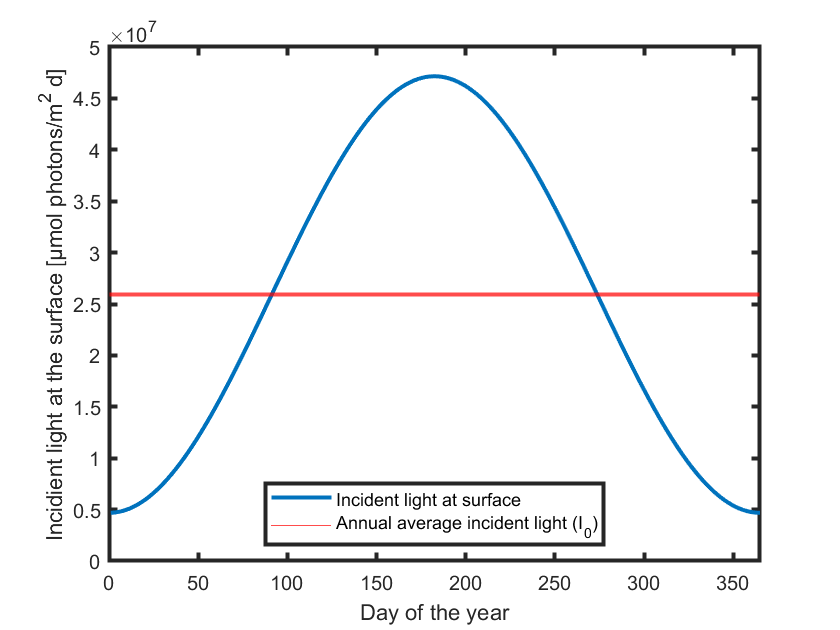
\includegraphics[width=\linewidth]{Pictures/Lightvariation.png}
  \caption{Annual variation in $I_{surf}$}
  \label{fig:Isurfvar}
\end{subfigure}%
\begin{subfigure}{.5\textwidth}
  \centering
  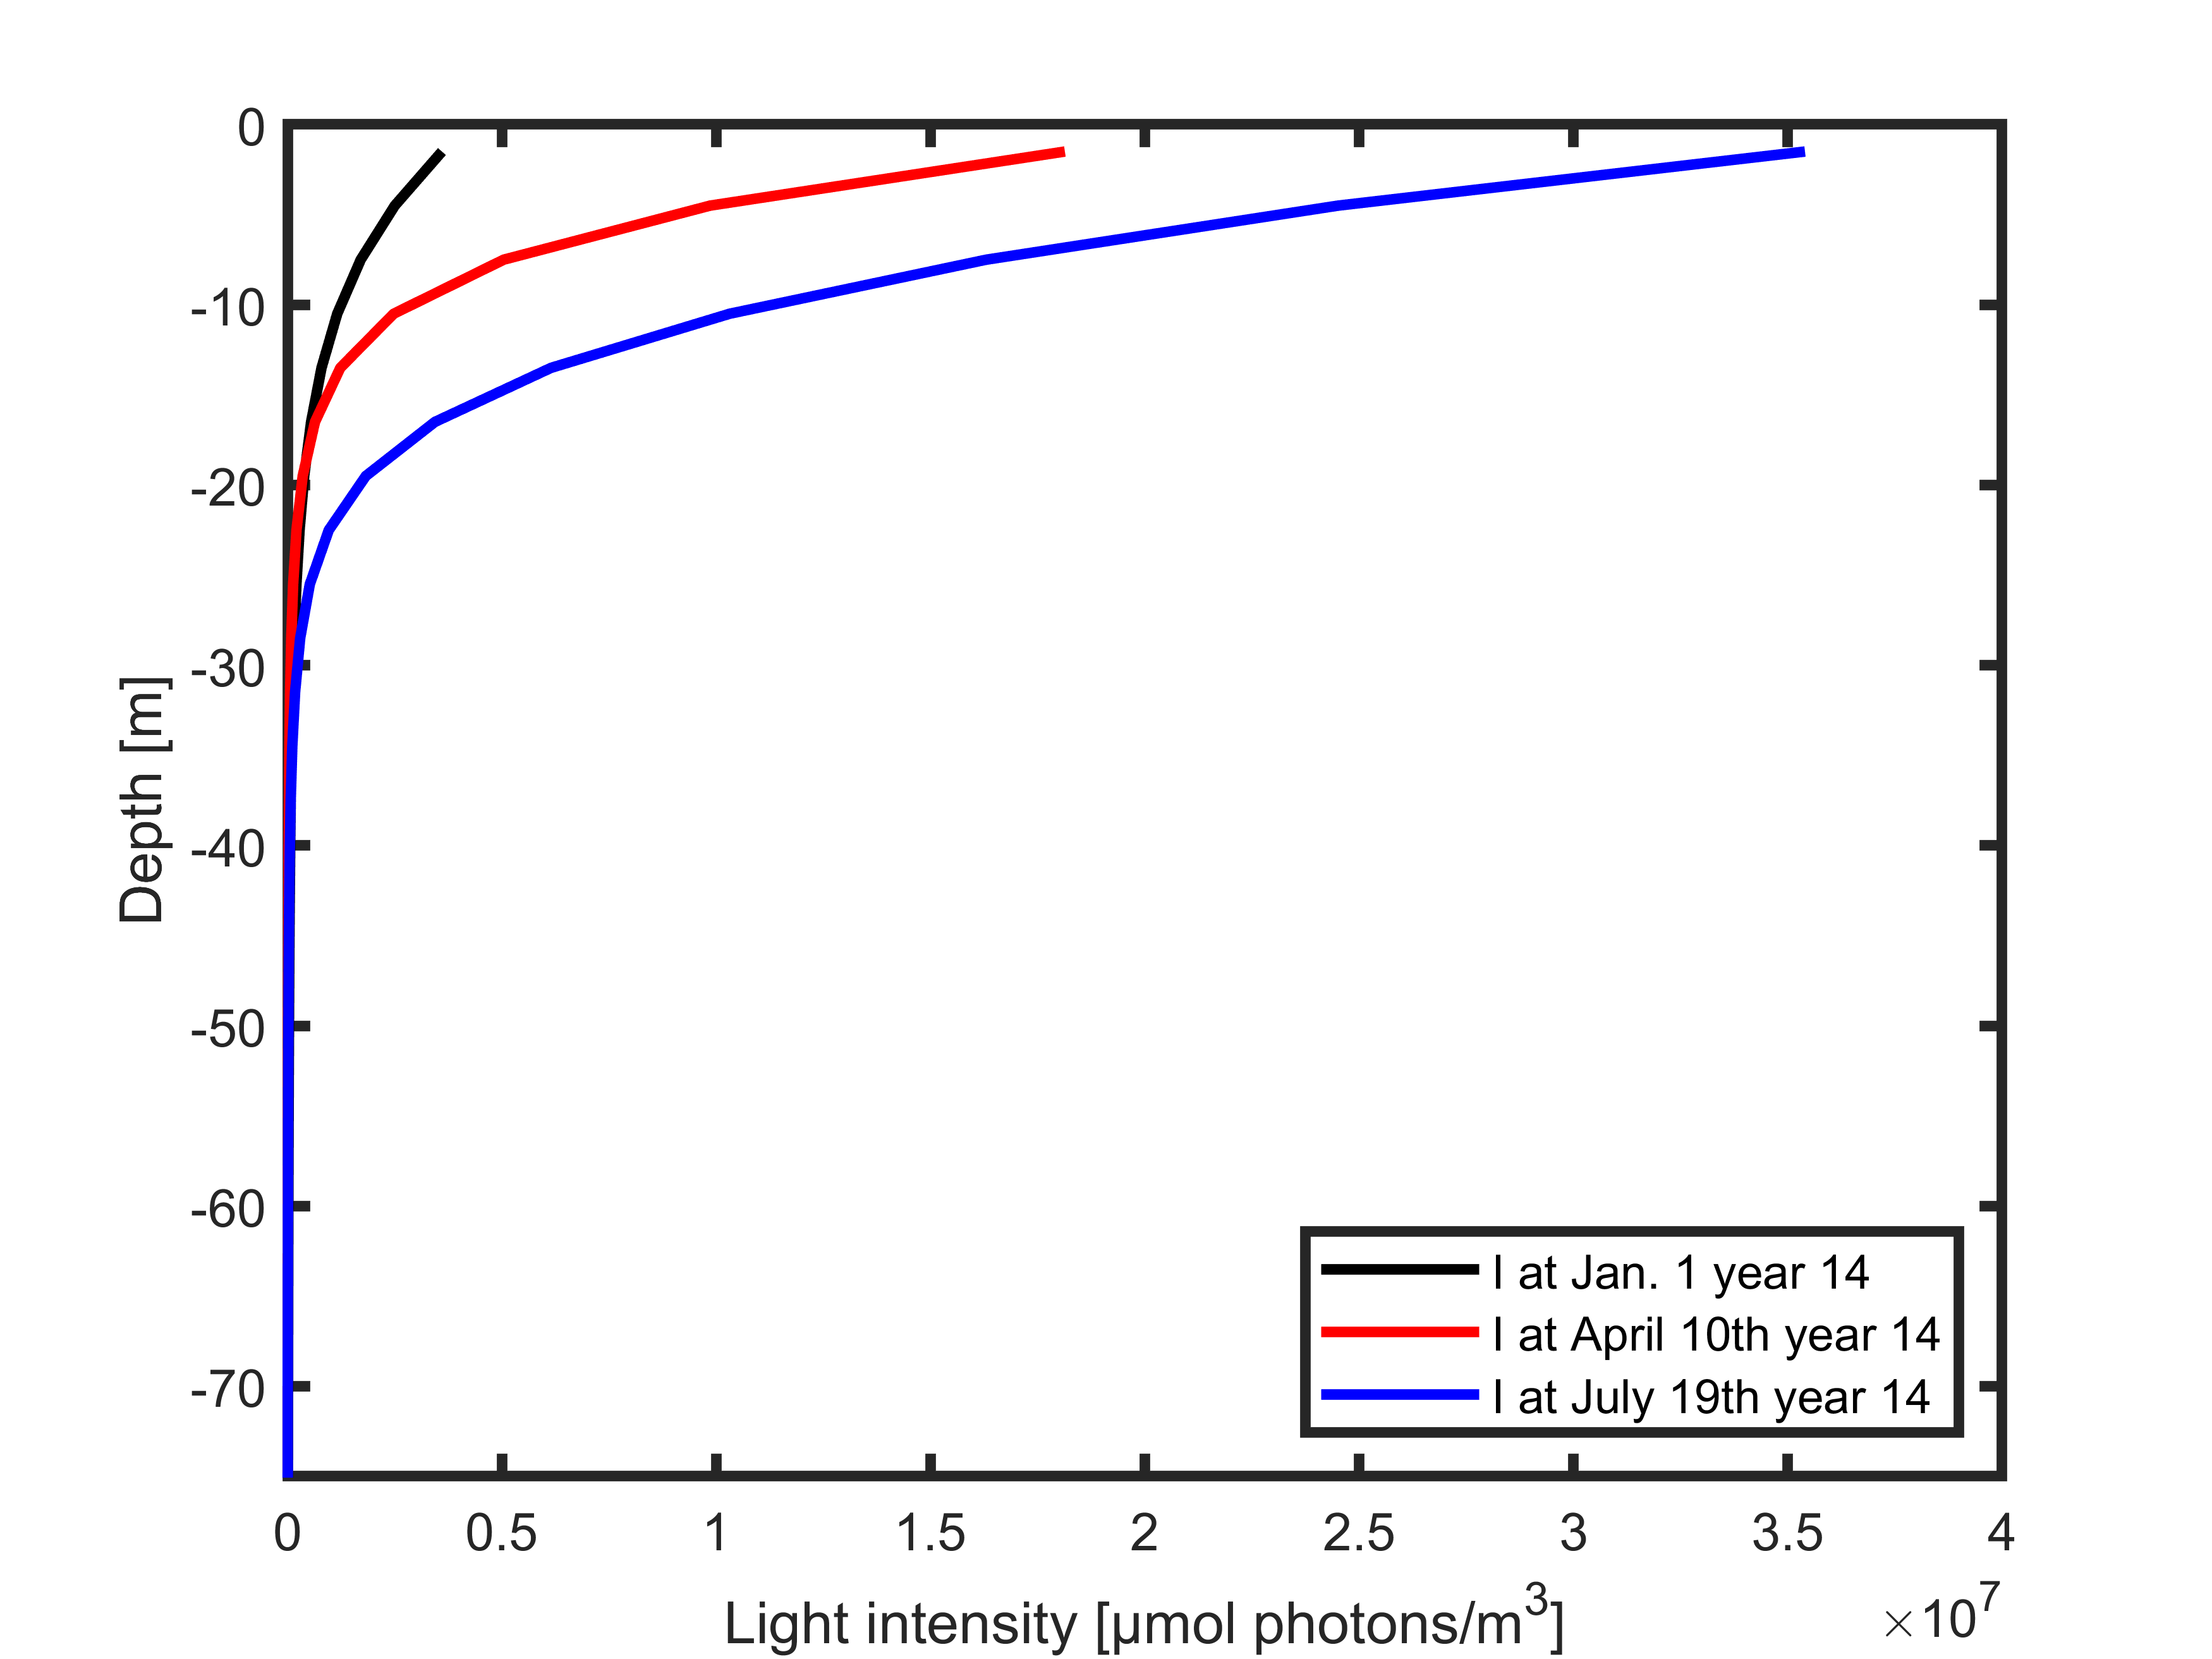
\includegraphics[width=\linewidth]{Pictures/ISeasonalVar.png}
  \caption{Impact of $I_{surf}$ on $I$ in the water column}
  \label{fig:Ivariation}
\end{subfigure}
\caption{The seasonal variations of incident light at the surface and its impact on the light intensity throughout the water column}
\label{fig:IandIsurfVar}
\end{figure}

To get a better understanding of annual variations, the model results for the last year (year 14), were plotted in its own 3D plot, \cref{fig:Y14Var}. From these 3D plots it is evident that there is enough nutrients available to produce a small bloom in the surface layer in spring, but the available nutrients gets depleted in the surface layer throughout the summer which forces the phytoplankton growth and maximum concentrations to sink to a depth of approximately 25-30 meters.    

\begin{figure}[h!]
\centering
\begin{subfigure}{.5\textwidth}
  \centering
  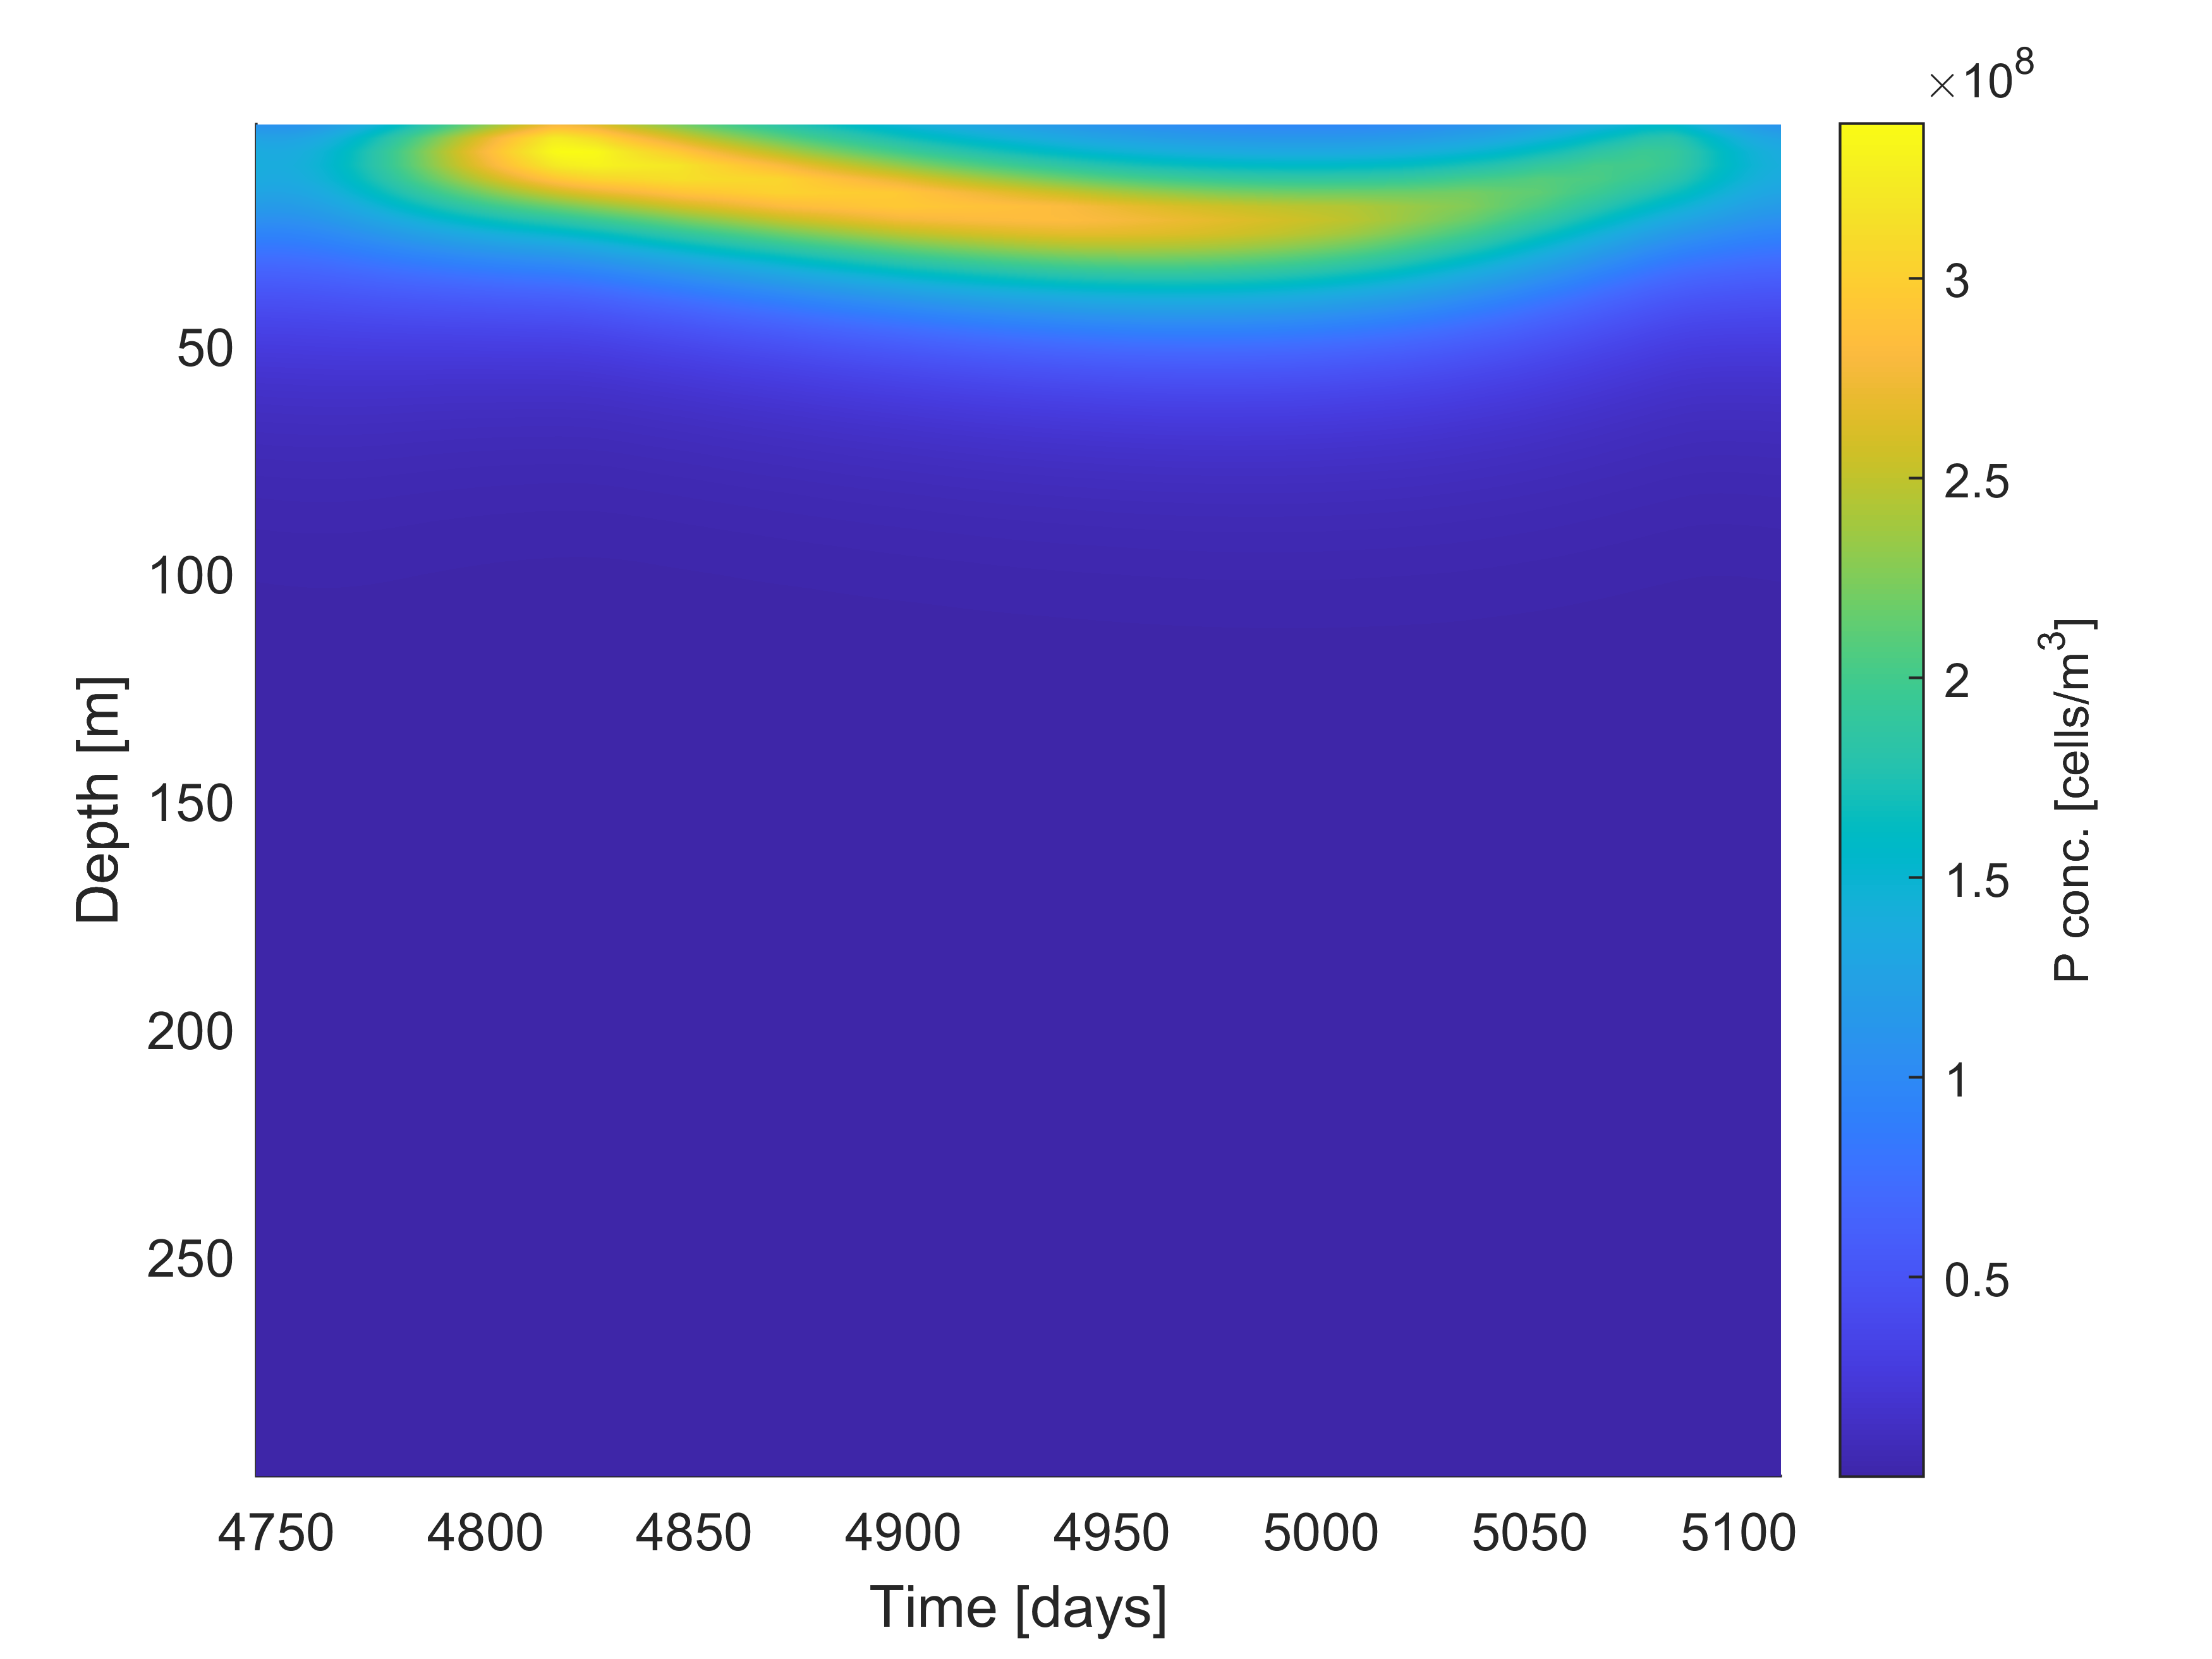
\includegraphics[width=\linewidth]{Pictures/Year14P.png}
  \caption{Annual variation in $P$ in year 14}
  \label{fig:Y14P}
\end{subfigure}%
\begin{subfigure}{.5\textwidth}
  \centering
  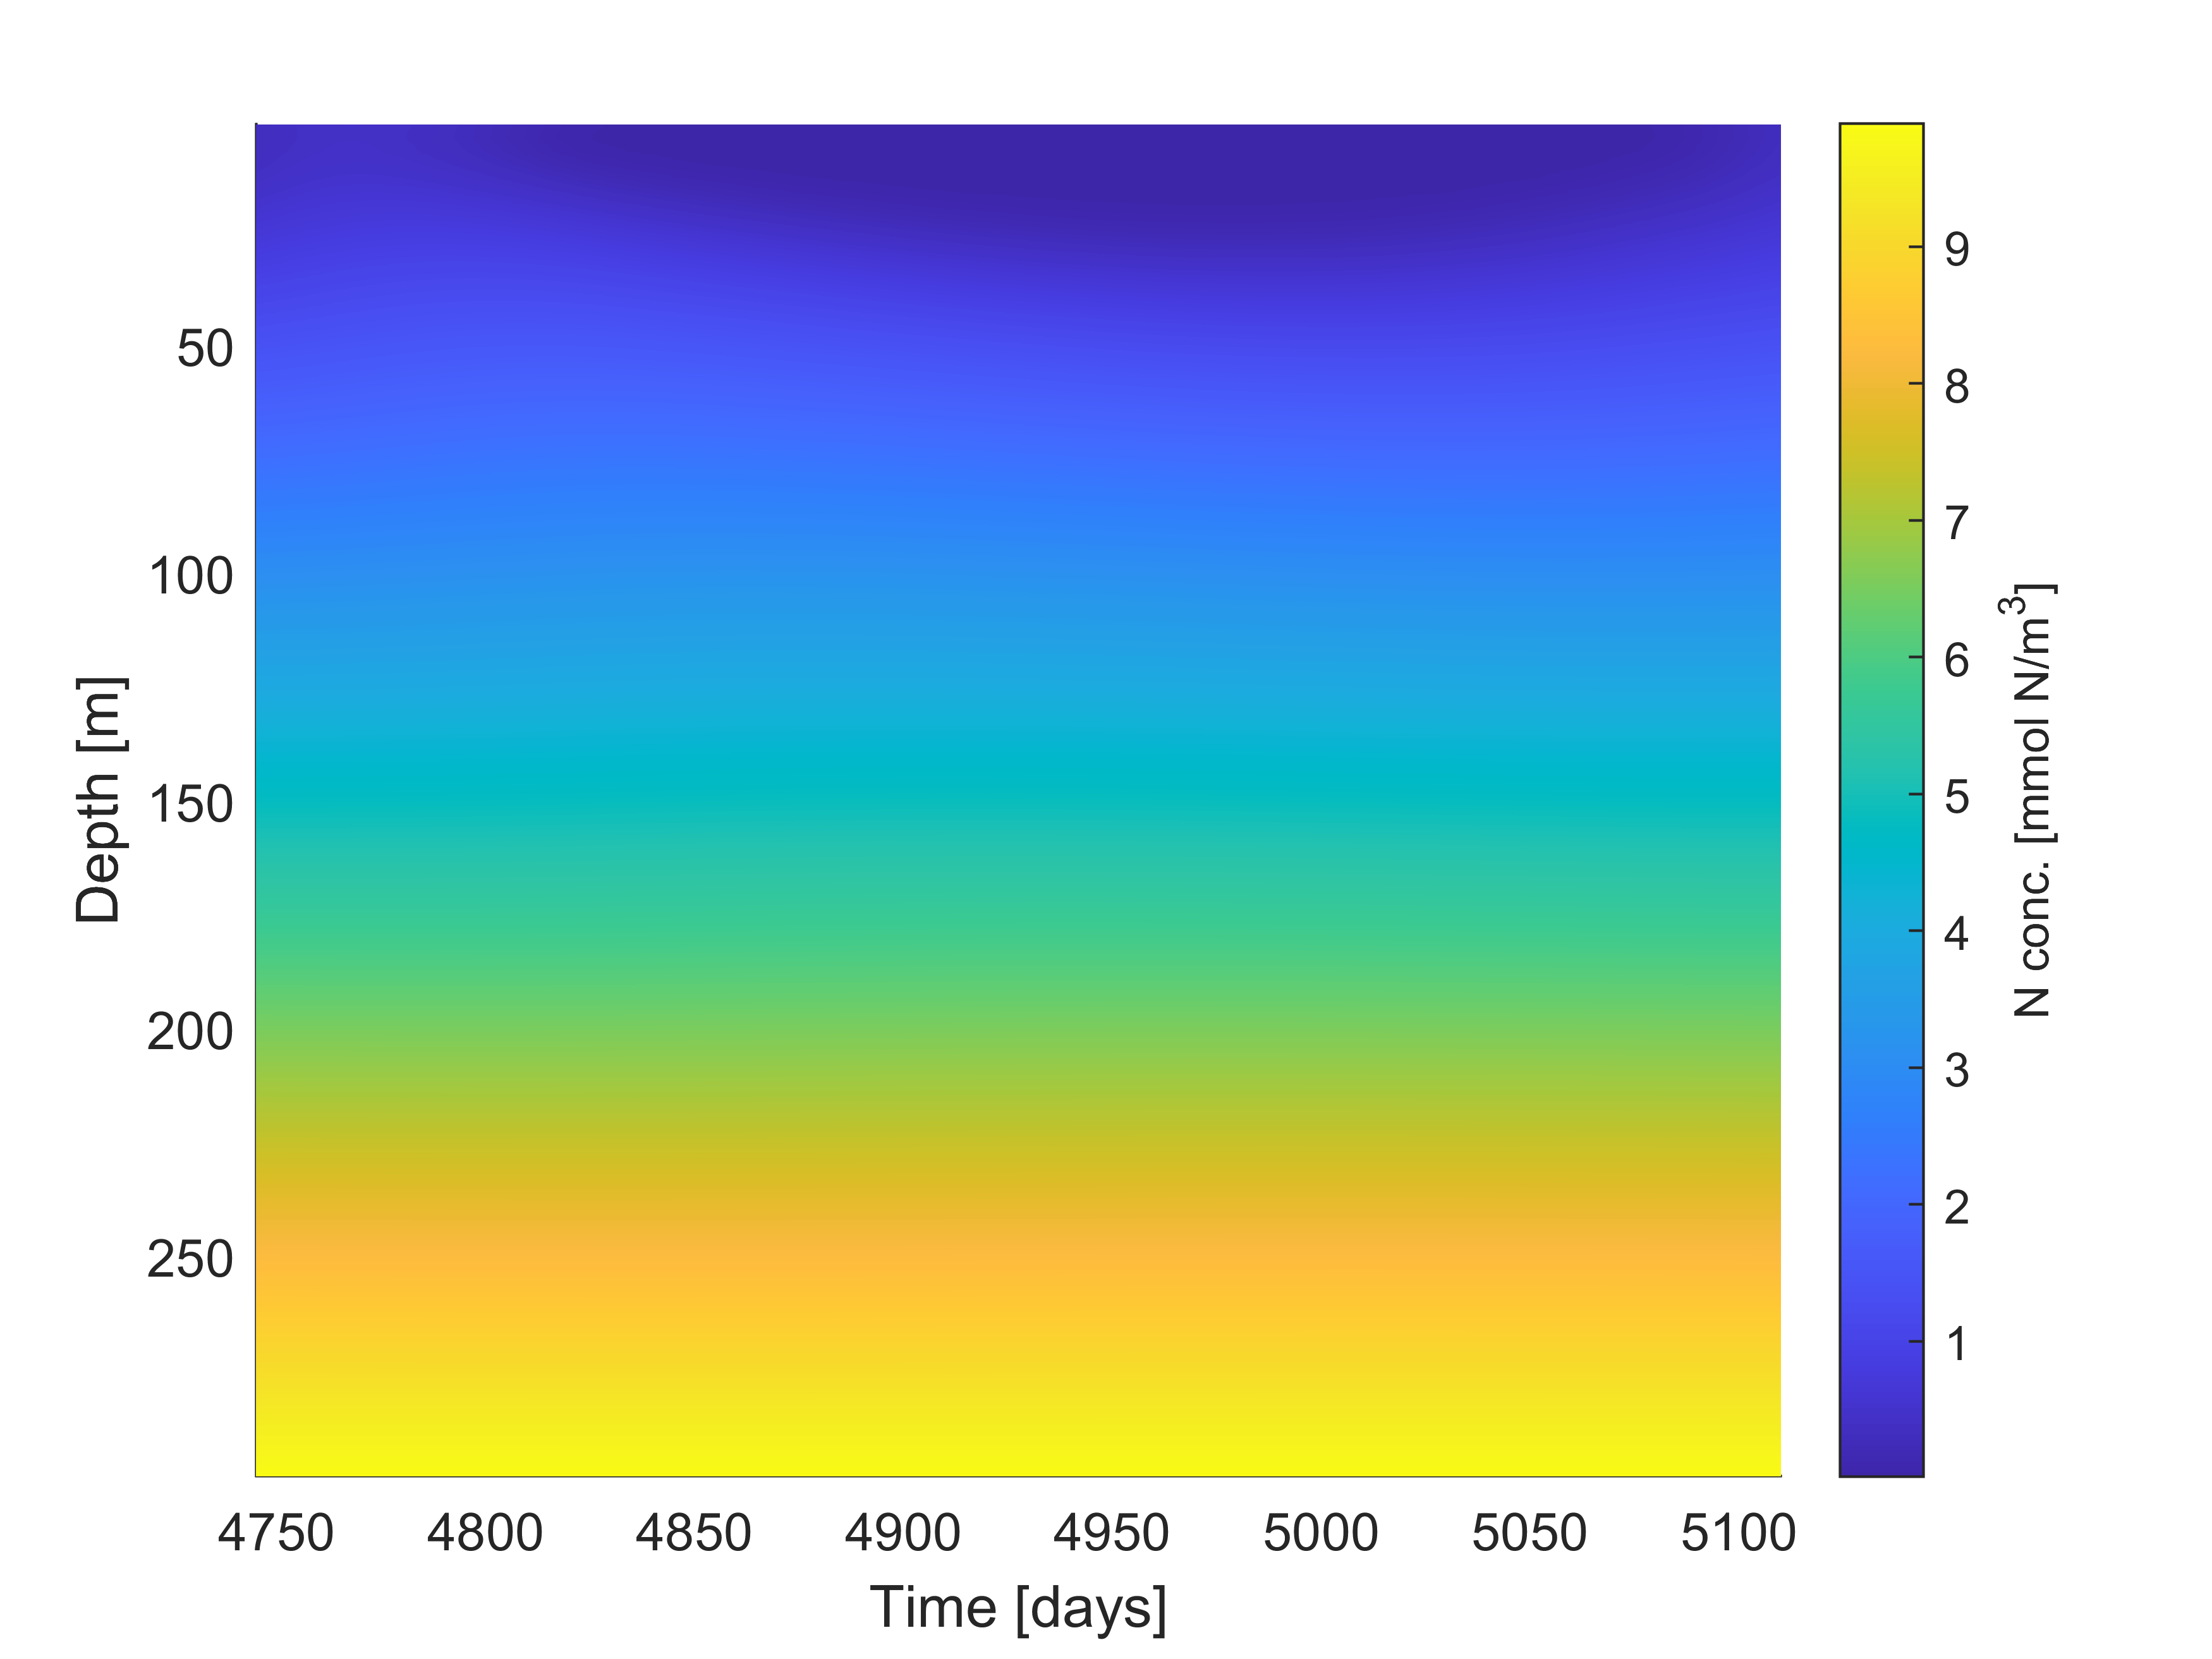
\includegraphics[width=\linewidth]{Pictures/Year14N.png}
  \caption{Annual variation in $N$ in year 14}
  \label{fig:Y14N}
\end{subfigure}
\caption{The annual variations of $P$ and $N$ in year 14}
\label{fig:Y14Var}
\end{figure}

\newpage
\section{Sensitivity analysis}
\subsection{Grid sensitivity}
After the initial base run of the model a sensitivity analysis were performed, starting with testing grid sensitivity. For all sensitivity analysis, the seasonality of incident light at the surface has been omitted, and $I(z,t)$ has been calculated using \cref{eq:Ieq2}. The model did not show much sensitivity to changes in grid sizes, and the small difference for the depth profile with a grid size of 6 meters is due to lower "resolution", \cref{fig:GridSens}.      
\begin{figure}[h]
\centering
\begin{subfigure}{.5\textwidth}
  \centering
  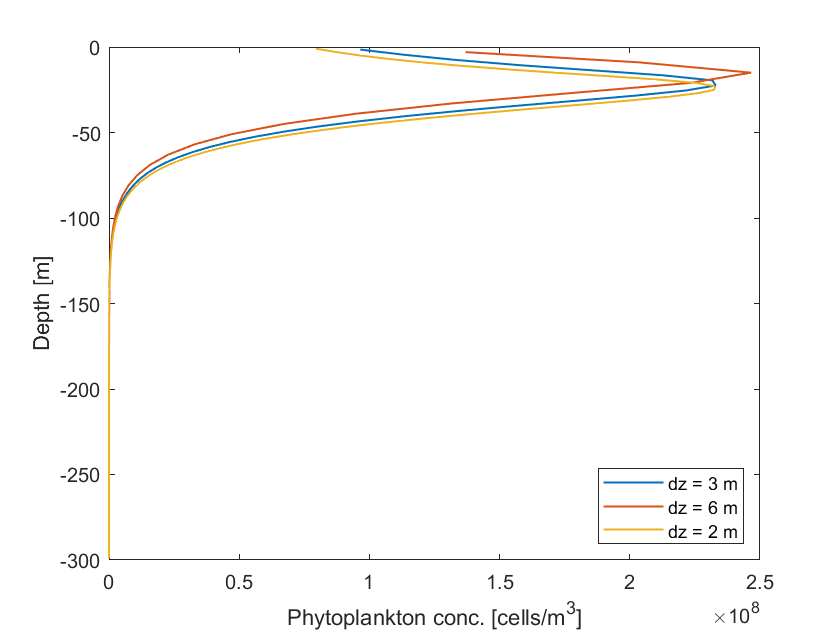
\includegraphics[width=\linewidth]{Pictures/Gridsensitivity.png}
  \caption{Grid sensitivity for phytoplankton}
  \label{fig:PGridSens}
\end{subfigure}%
\begin{subfigure}{.5\textwidth}
  \centering
  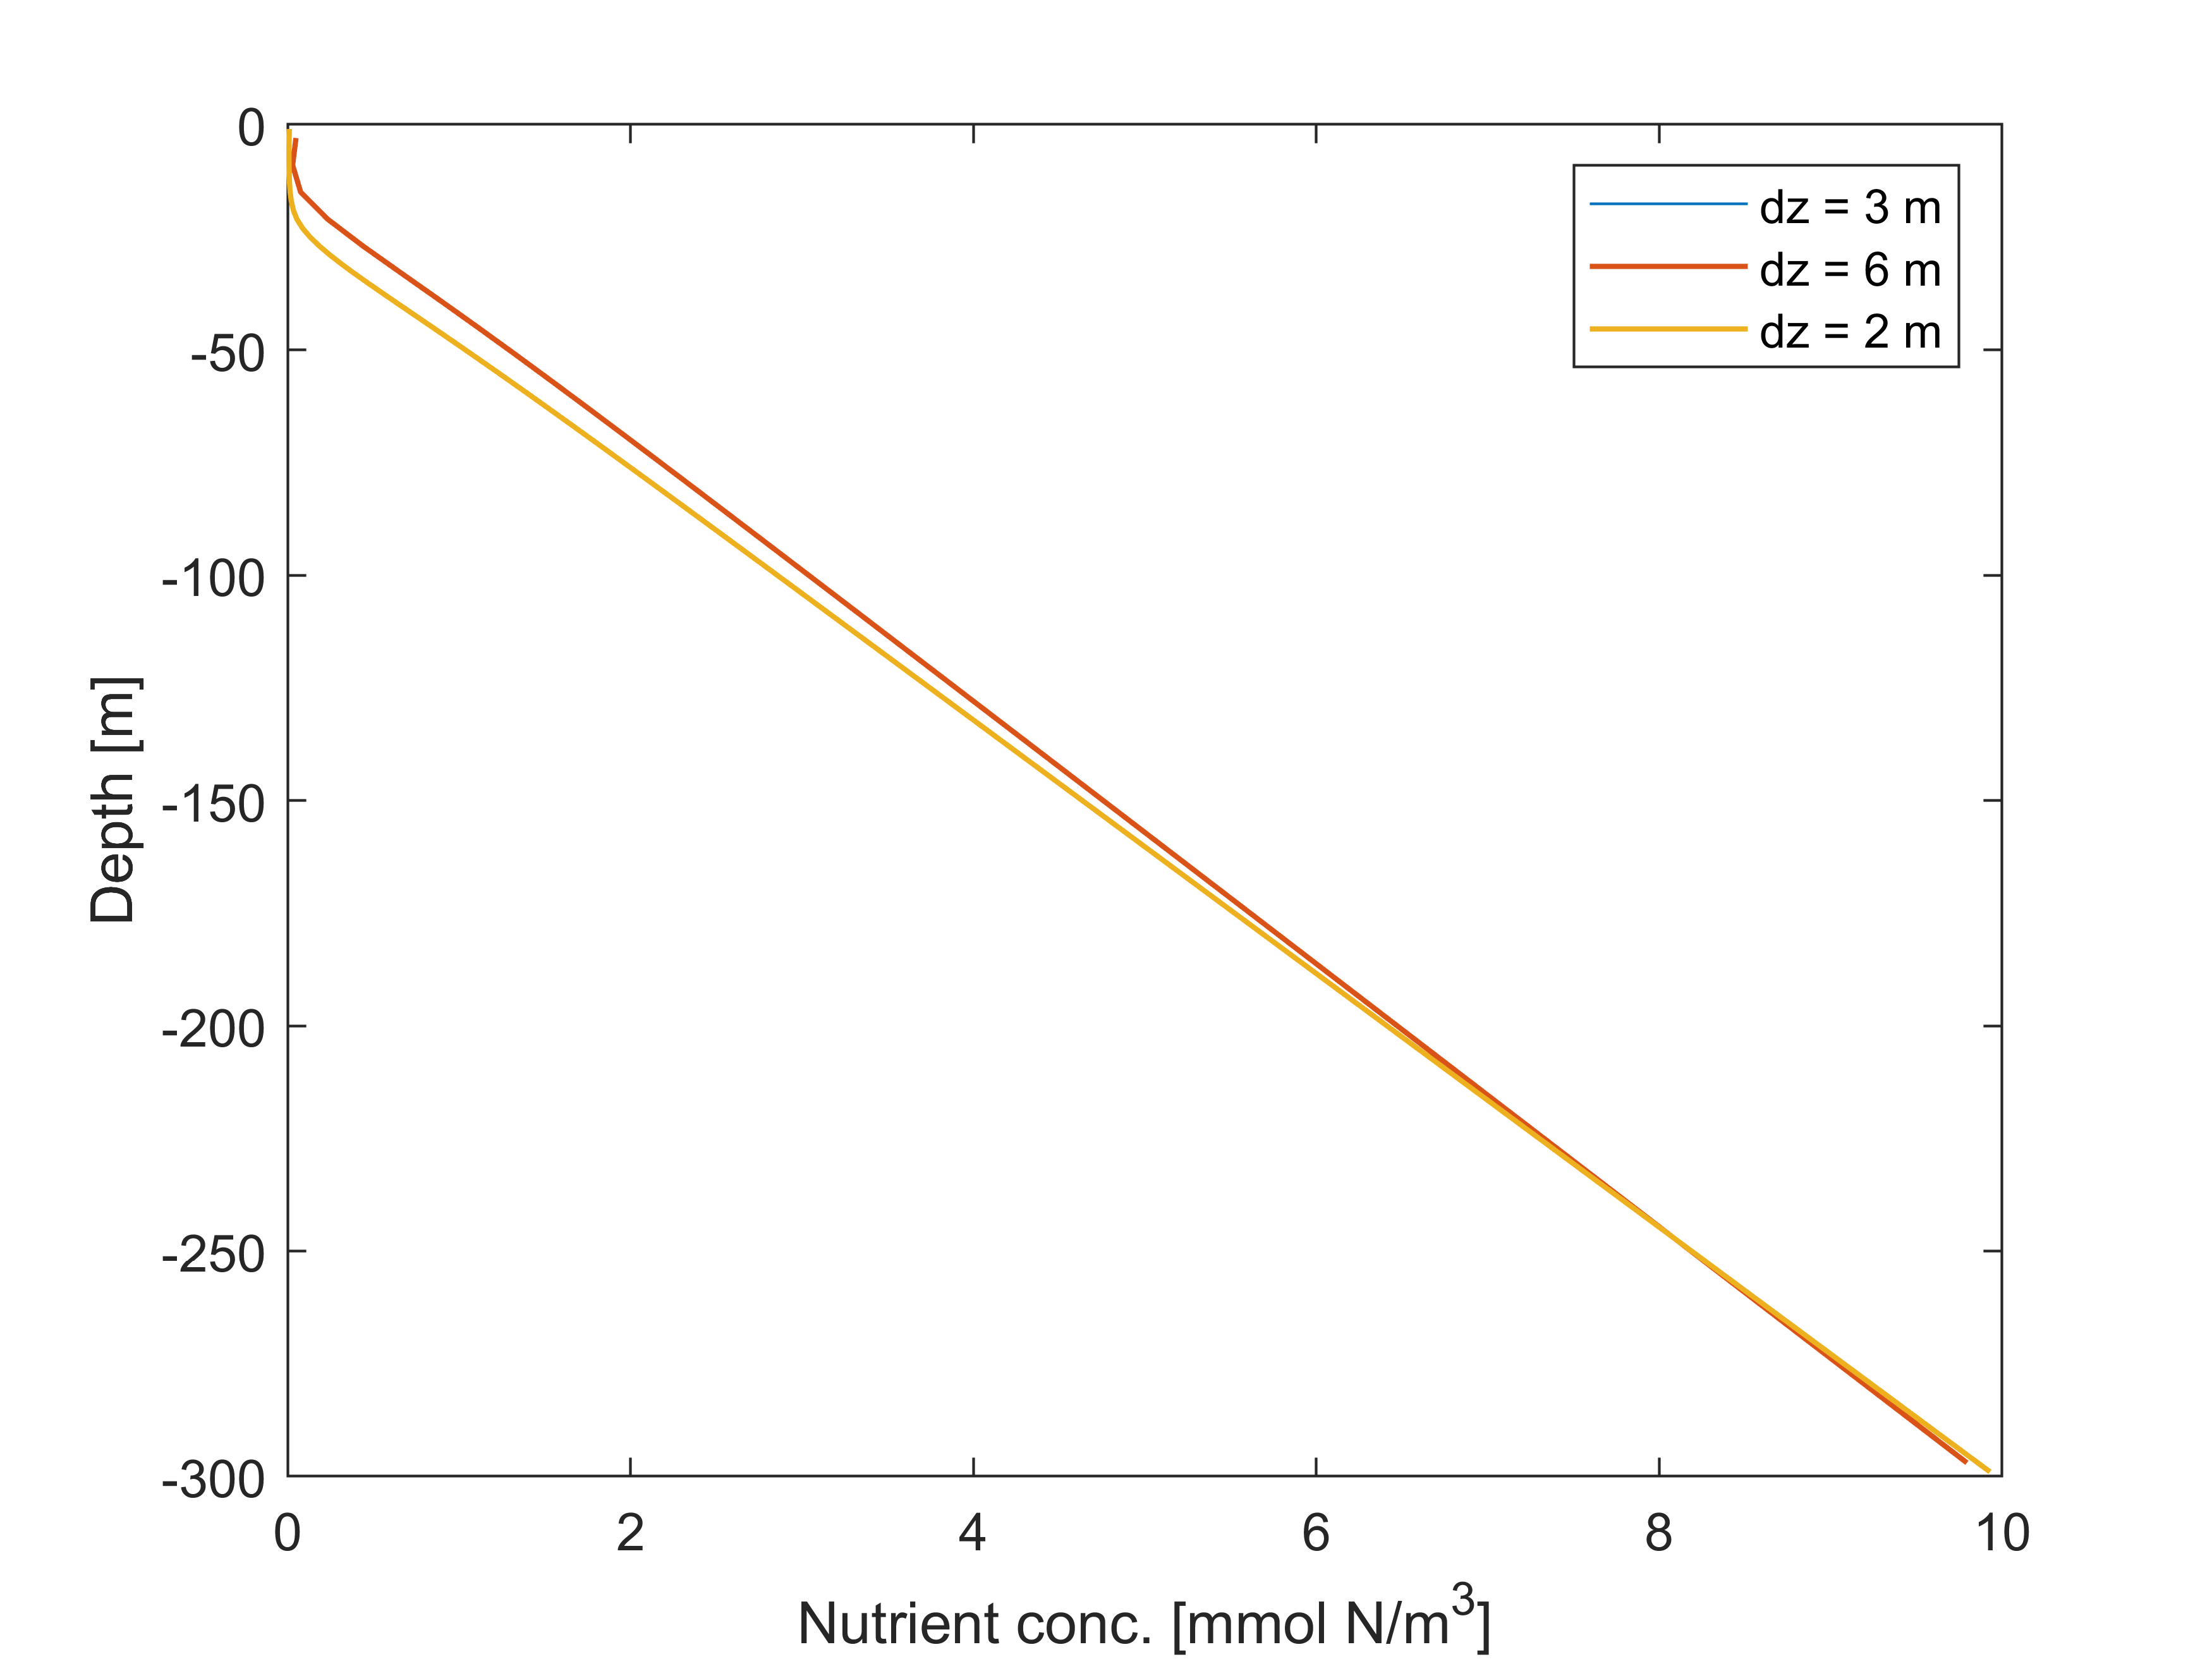
\includegraphics[width=\linewidth]{Pictures/GridsensitivityN.png}
  \caption{Grid sensitivity for nutrients}
  \label{fig:GridSensN}
\end{subfigure}
\caption{Grid sensitivity for both P (a) and N (b), by changing $dz$ between 2, 3 (as in base run) and 6 meters.}
\label{fig:GridSens}
\end{figure}

\subsection{Sensitivity of chosen parameters}
Sensitivity analysis were also performed for a few chosen parameters. Among those are the constant diffusivity, $D$, which was a constant of 30 $m^2/d$ in the base run. As seen in \cref{fig:DSens}, both lowering and increasing the diffusivity leads to changes in the maximum phytoplankton concentration and the depth to which this maximum is present. Lowering the $D$ to 10 leads to a much deeper maximum of phytoplankton at approximately 200 meters depth, while the maximum concentration is also much larger. While increasing $D$ to 50, lead to a slightly higher maximum at approximately 10 meters depth while the concentration again is much larger. This causes some concern about the parameter $D$, and a further examination of why this parameter seems to have such large impact on the phytoplankton movement and concentration size.
The impact of $D$ is a result of increased vertical movement upwards when increased. Since $D$ is the same for both nutrients and phytoplankton, a low $D$ value of 10, leads to little nutrients diffusing upwards from the bottom, which results in the maximum phytoplankton concentration being at a depth of 200 meters. 
\begin{figure}[h]
\centering
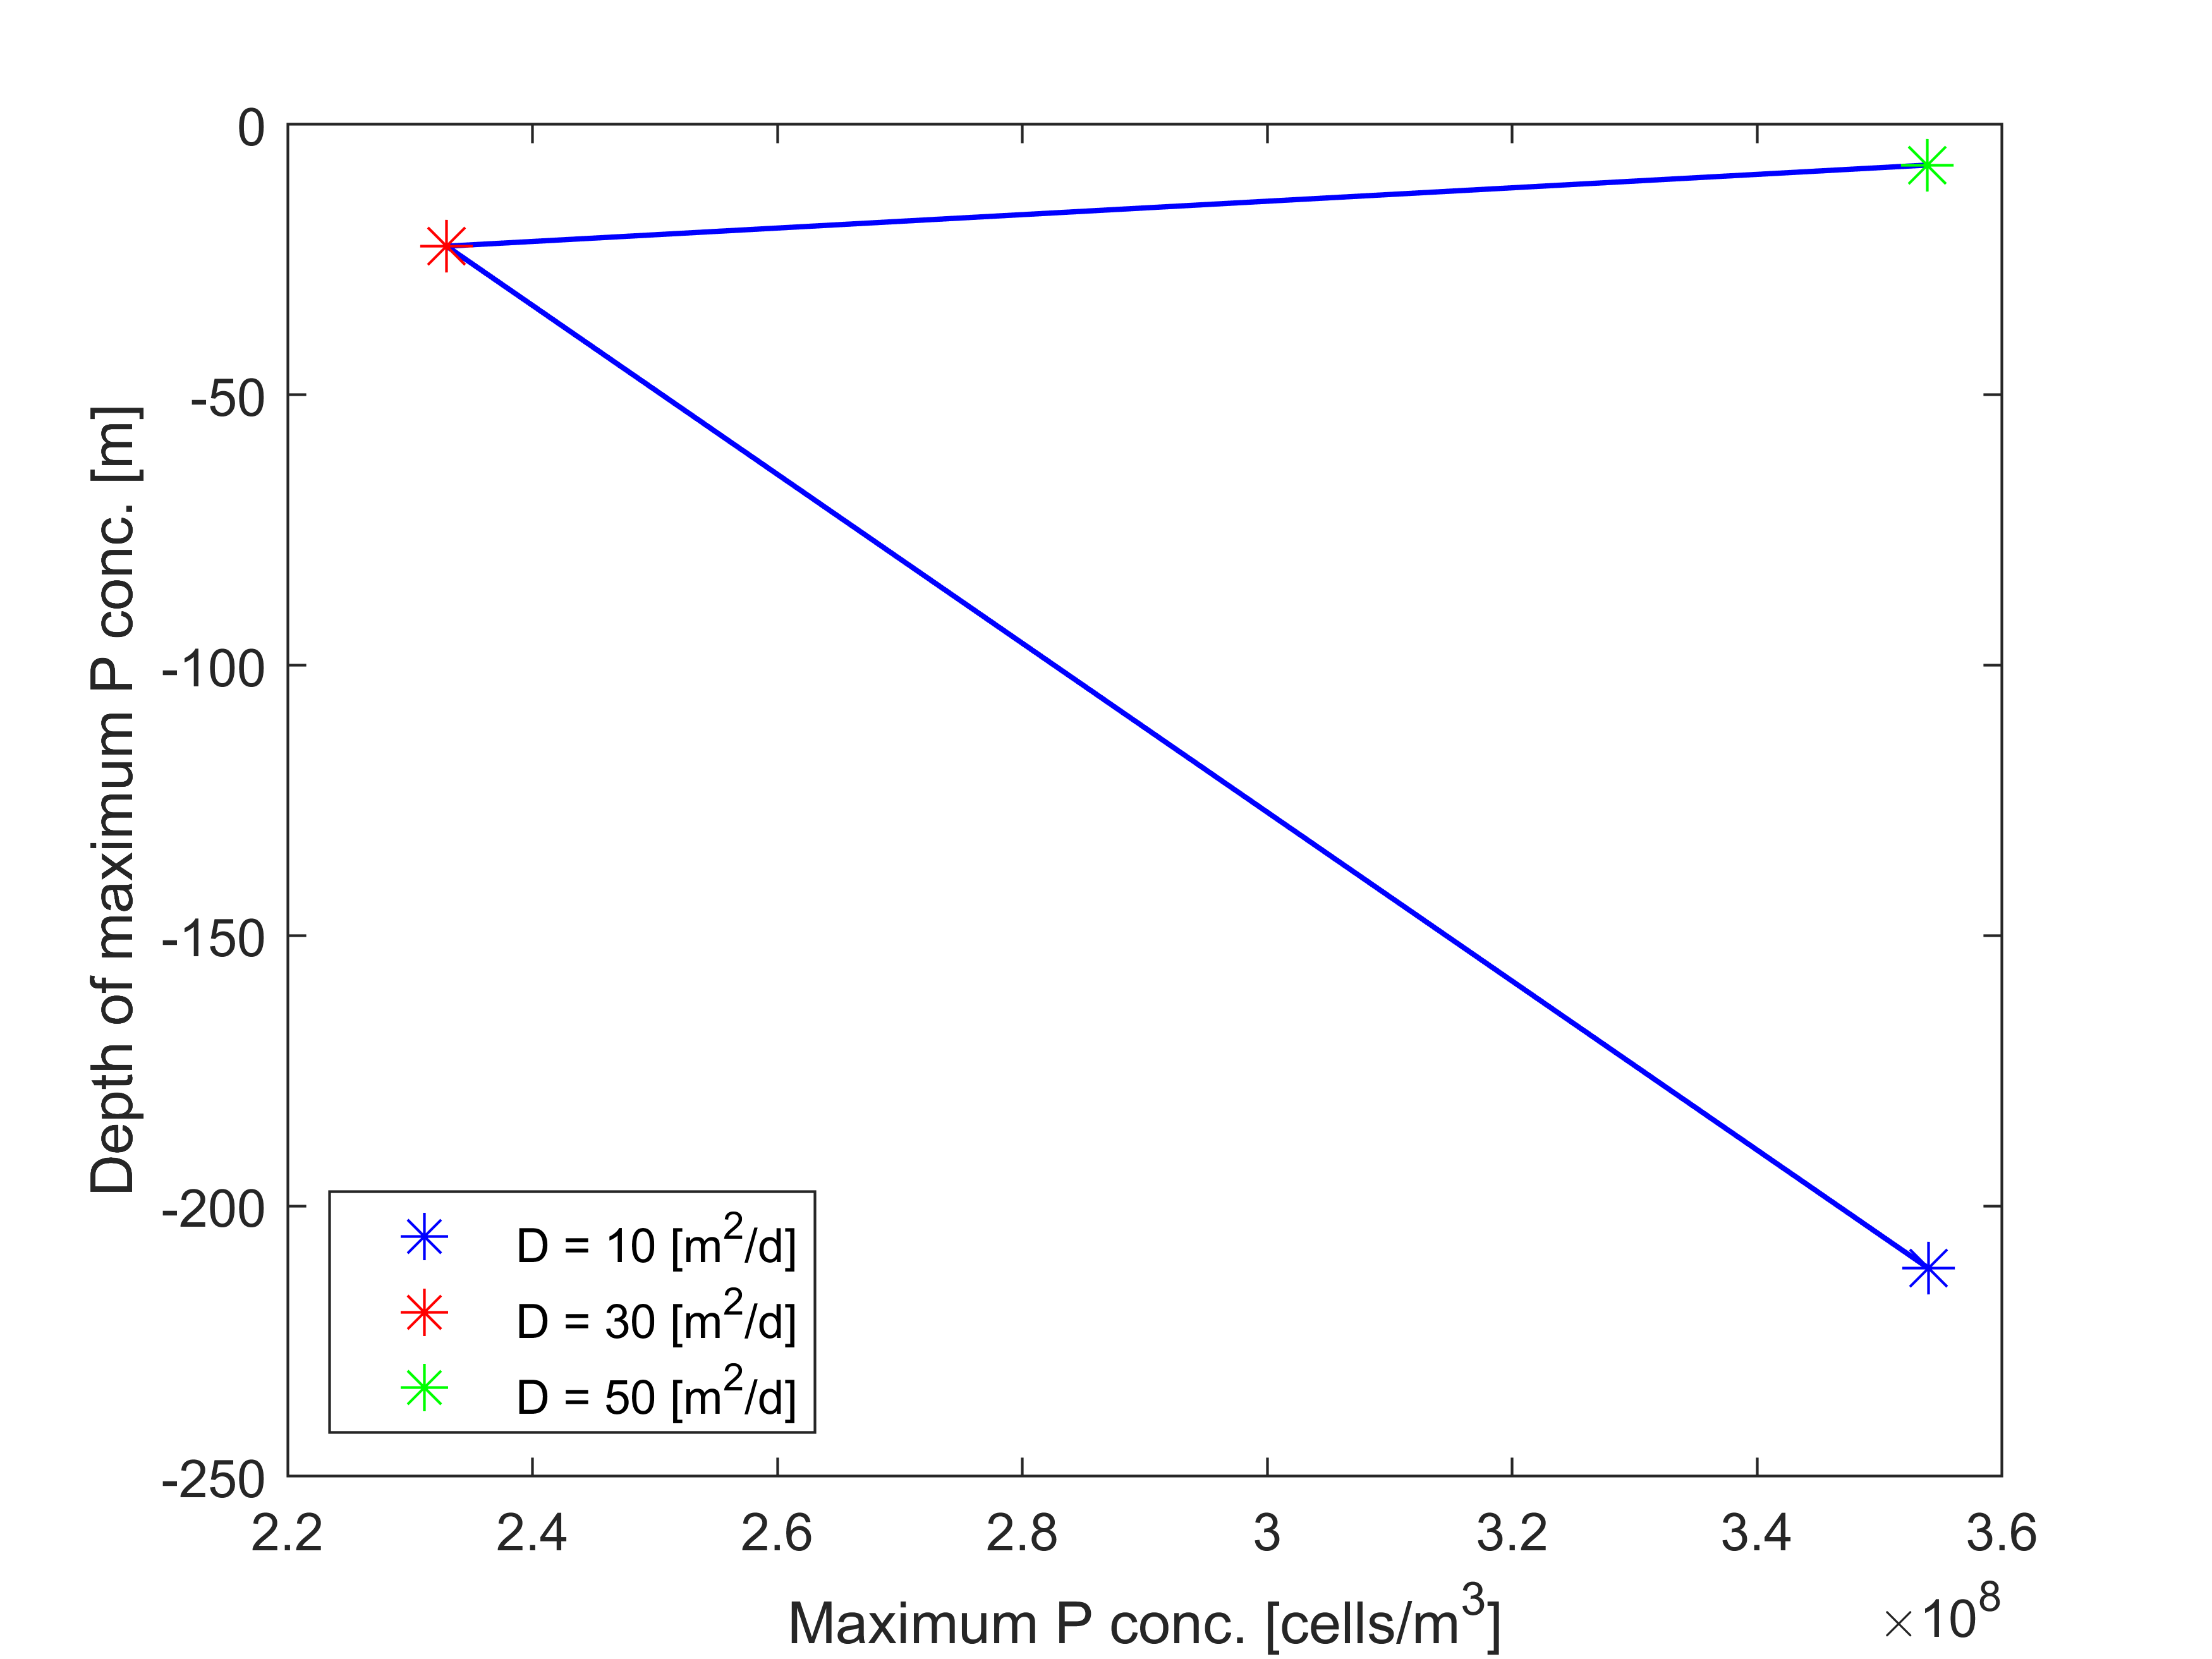
\includegraphics[width=\linewidth]{Pictures/Dsensitivity.png}
\caption{Sensitivity of phytoplankton conc. when changing the constant diffusivity $D$}
\label{fig:DSens}
\end{figure}

\newpage
\section{Limiting factors}
In this section, the two limiting factors of either nutrients or light intensity will be examined.
The growth factor of phytoplankton, $\mu$ is limited by either nutrient or light intensity, based on von Liebig's law of minimum as described in \cref{eq:Growtheq}. The two growth limiting terms of the equation is plotted in \cref{fig:Limit}. As it can be seen, the maximum concentration of pythoplankton is located slightly below the depth at which the two limiting terms crosses each other at around 22 meters depth. At around 25 meters depth, the light limiting growth crosses and becomes smaller than the net zero growth, $\frac{l}{\mu_{max}}$, given by the dashed vertical line. This means that although there is plenty nutrients available, von Liebig's law of minimum imposes that the lack of light makes it impossible for phytoplankton to grow, which is why we see the decreasing phytoplankton concentration at depths below this point.  
\begin{figure}[h!]
\centering
\begin{subfigure}{.5\textwidth}
  \centering
  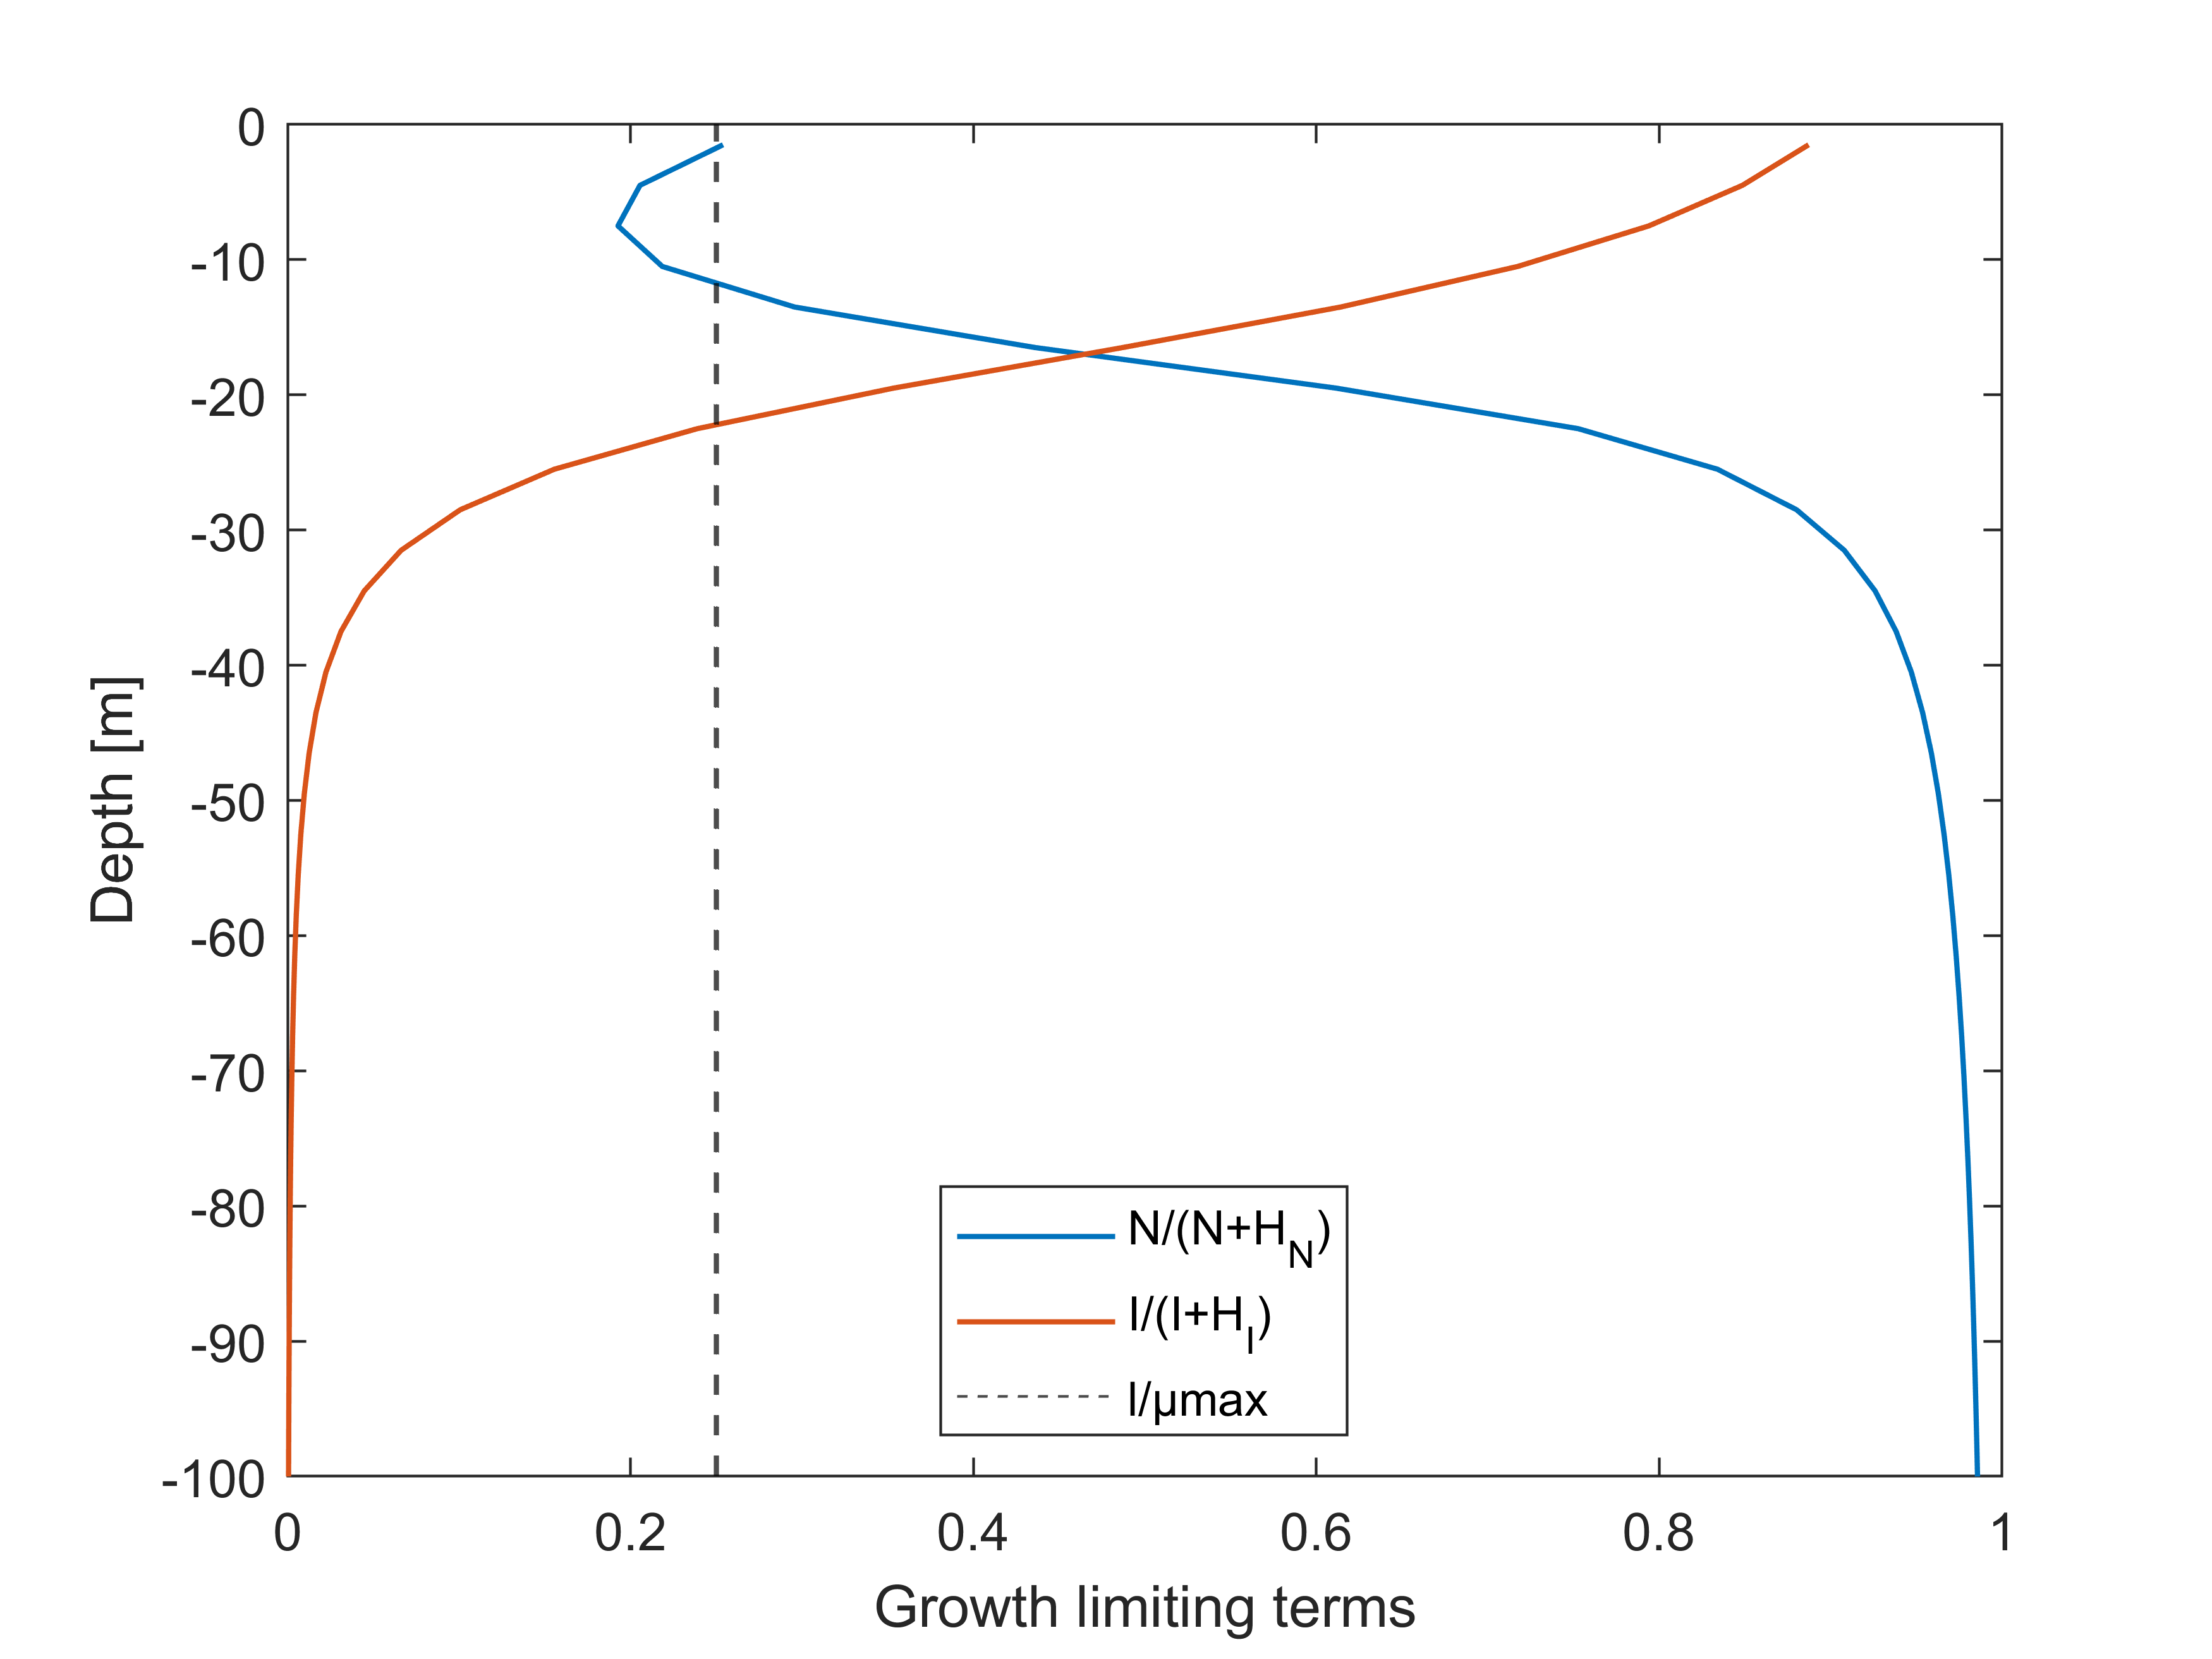
\includegraphics[width=\linewidth]{Pictures/Limitingfactor.png}
  \caption{Limiting growth terms of \cref{eq:Growtheq}}
  \label{fig:LimitingFac}
\end{subfigure}%
\begin{subfigure}{.5\textwidth}
  \centering
  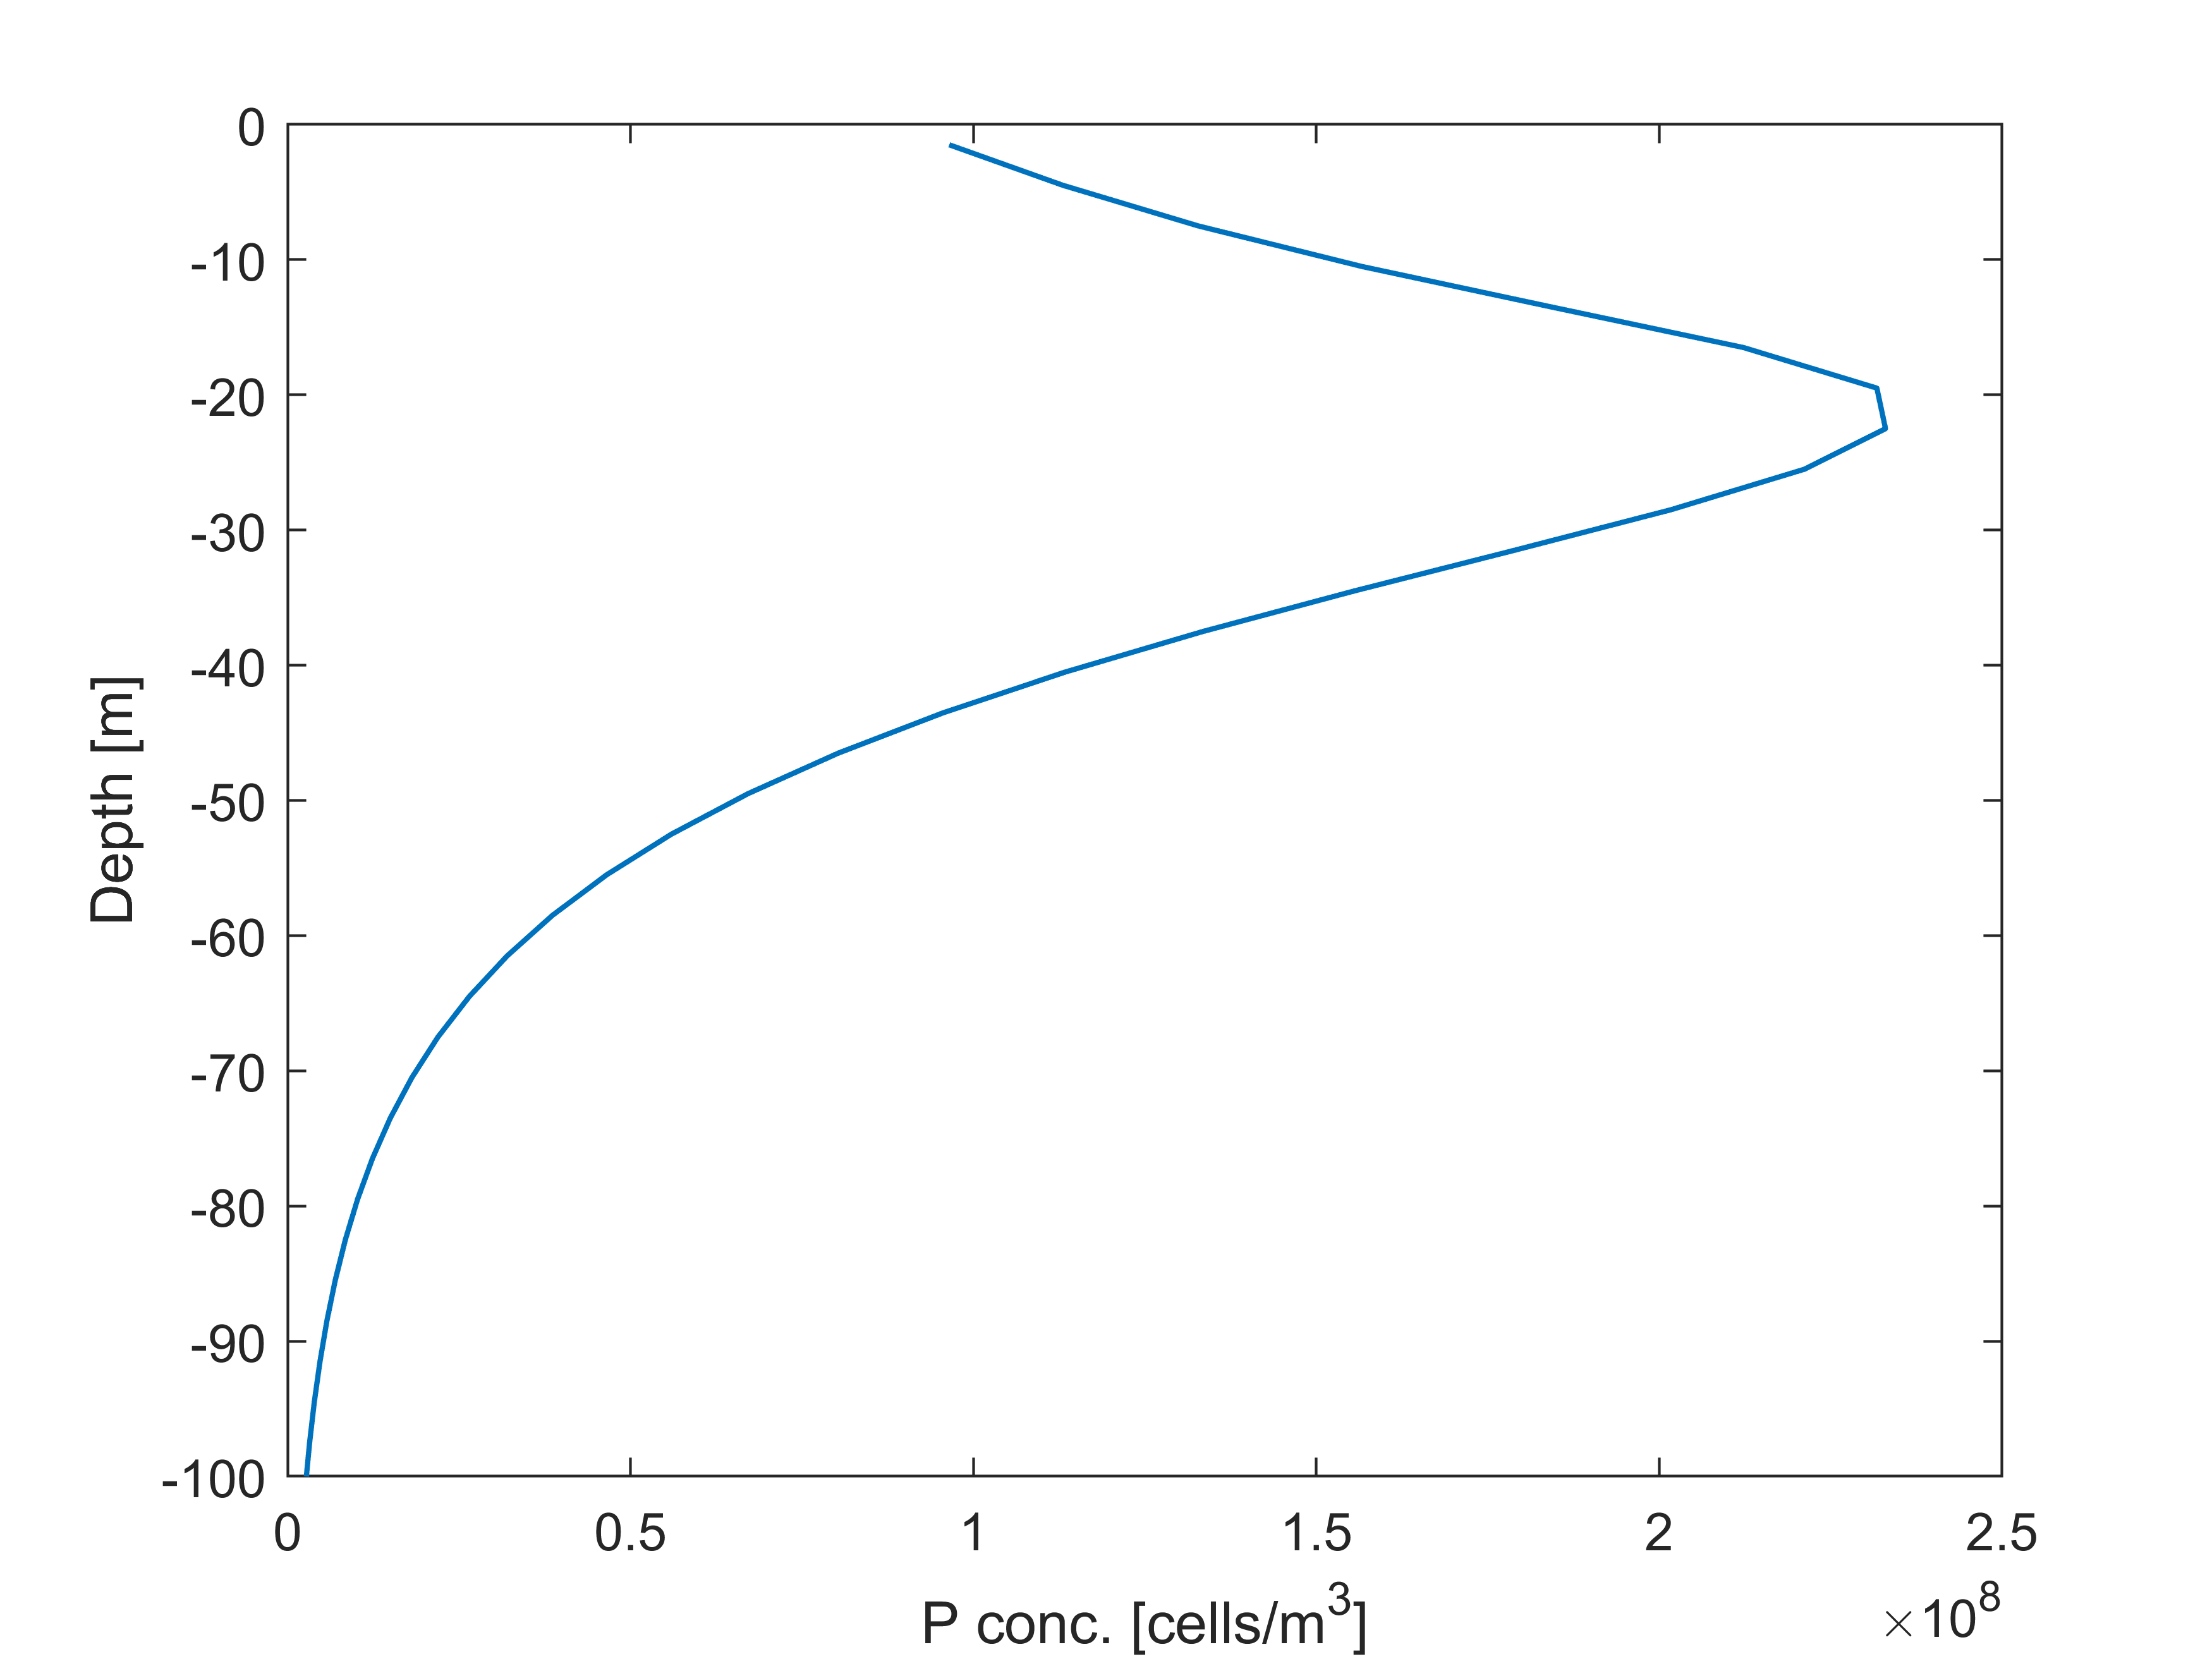
\includegraphics[width=\linewidth]{Pictures/LimitingfactorPplot.png}
  \caption{The accompanying P conc.}
  \label{fig:LimitingFacP}
\end{subfigure}
\caption{An overview of the limiting factors and the P conc.}
\label{fig:Limit}
\end{figure}